\documentclass[a4paper,12pt]{article}

\title{\textbf{Visualization}: Exploring library dependencies in modern software projects\\\emph{Midway report}}
\author{Ask Neve Gamby, Rune Filtenborg Hansen,\\
Henrik Urms, and Niels Gustav Westphal Serup}

\usepackage[T1]{fontenc}
\usepackage{lmodern}
\usepackage[utf8]{inputenc}
\usepackage[british]{babel}
\usepackage{microtype}
\usepackage{underscore}
\usepackage{amsmath}
\usepackage{graphicx}
\usepackage[hidelinks]{hyperref}

\setlength{\parskip}{1ex}
\setlength{\parindent}{0pt}
\setlength{\parfillskip}{30pt plus 1 fil}

\begin{document}

\maketitle

\section{Introduction}

This project is about getting an overview of the structure of depended-upon code
in a large software project, and help developers make informed decisions about
what software libraries (not) to use.


\subsection{Related Work}

We have looked at a series of articles to determine what could quantitatively
describe a ``good'' software library.  While we still need to work on that
definition, we have looked at a few papers, these investigate different parts at
visualizing sofware dependencies.

Their main goal is to discern the dependencies from classes and objects. The
papers assert that the typical representation of depencies in software is made
using graph structure.  The articles try to present new ways of representing
such graphs.

The first
paper\footnote{\url{http://www.tzi.de/st/papers/domtree-vissoft05.pdf}} uses a
specific sort of tree to filter the amount of nodes down to a smaller subset
such that it becomes clearer from a user perspective to understand the
visualization. This is important as the number of nodes can become overwhelming,
though we suffer some information loss using this method.

The second
paper\footnote{\url{http://rmod.inria.fr/archives/papers/Berg14a-Vissoft-DomainSpecific.pdf}}
proposes a new graph constructing language, to help creating visualizations
showing graphs. This new graph language is argued to be more efficient in both
layout and setup, as it can take several arguments at a time, instead of
specifying each argument.  This method uses different channels to encode the
properties of the dependency graph it shows. It uses color to map different
categories and size to mark the usage of these.


\section{Dataset}

Our datasets include the approximately 2000 Haskell programming language
packages on the Stackage dependency manager at \url{https://www.stackage.org/}.

For each package it is possible to get the following attributes:

\begin{itemize}
\item The name.
\item The version.
\item What software modules it exposes (only relevant if the package is a
library).  (In Haskell, a package can have more than one module.)
\item What modules it imports.
\item Its dependency dictionary.  Each key-value pair in the dependency
dictionary consists of the package name of the dependency (the key) and a list
of the modules from that package in use (the value).
\end{itemize}

The dataset is located here for the current snapshot (internally consistent list
of packages) of the Haskell packages:
\url{https://raw.githubusercontent.com/nqpz/vis-dependencies/master/data/lts-7.3.json}


\section{Tasks}

\subsection{Target Group}

Our target group can be describes as developers of modern software, more
specifically developers interested in improving whatever project they are
working on.  This especially includes:

\begin{itemize}
\item Developers having done lots of code sprints over a period of months, and
now want to take more thorough look at the code as a whole.
\item Developers taking over as maintainers of a new project in need of
refactoring.
\end{itemize}

\subsection{Goals}

\begin{itemize}
\item Identify packages to Add, Remove or swap out for other packages in project a while restructuring or rewritting some of the code.
\end{itemize}

\subsection{Domain}

To aid these developers, it would be nice to show them all kinds of stats about
a software project.  To limit ourselves, we have chosen to only show the effects
of the dependencies.

Using the attributes of each package in the dataset, we would like to show our
definition of a healthy package, and how much each dependency is used.

We can also show conflicts between dependencies.  This should not be a problem
for packages on Stackage, but it might happen for local, untested projects where
packages are added and removed rapidly during development.  This is also solved
with conventional command-line tools, but can be nice to show in a visualization
as well to get a more complete picture.


\section{Design}

We have included a design sketch in figure~\ref{fig:sketch0}.

\begin{figure}[h!]
\begin{center}
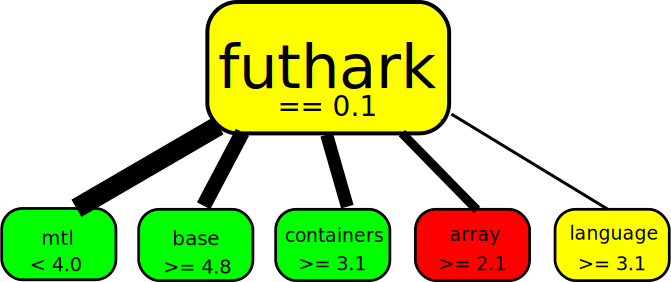
\includegraphics[width=0.8\textwidth]{sketch0.pdf}
\caption{A sketch of the visualization.}
\label{fig:sketch0}
\end{center}
\end{figure}

In this sketch, the main package ``futhark'' that we want to inspect is at the
top, and its dependencies are at the bottom.  Each package has a color
describing its maturity.  When you click on the package, the attributes
determining the maturity should be expanded and described.

Instead of lines with varying sizes, we could also vary the sizes of the the
dependency boxes, and not care that much whether they are located perfectly
below the main package.  This might make the visualization easier to implement
and still provide enough visual clues.

The visualization could also be expanded to show conflicts between dependencies
as e.g. dotted lines, since this is also useful knowledge.

\subsection{Measuring the Maturity}

We would like to measure the maturity of a package dependency, i.e. its
stability, so that we can give it a proper color in the visualization.  We have
access to the following attributes:

\begin{itemize}
\item The number of reverse dependencies of a package.  There might be a
correlation between a package being popular and that same package being mature,
and we can use this attribute to determine popularity.
\item In some cases it is also possible to see how many people have contributed
to the package, although this is only the case if the package includes a link to
its source management system page, e.g. a GitHub page.  This is not currently
included in the linked dataset, but we can extract the information and include
it if we decide to.
\end{itemize}

We are still working on defining this attribute based on experiences in the
literature.


\section{A Scenario: Getting an Overview}

This scenario describes the case where a large open source software project has
received a new maintainer.  Due to years of uncoordinated additions to the code,
the new maintainer would like to clean up.  This clean up involves removing
little-used packages.  The maintainer uses our visualization, initially focusing
on their own project package.  They notice some little-used, little-mature
dependencies, click on each of them, and try to figure out through normal means
whether these borderline-okay dependencies can be replaced.


\section{Implementation}

We expect to program the visualization in D3.js.


\end{document}
